\section{System Design and Demo Walkthrough}
\label{sec:system}

\begin{figure*}[t]
\centering
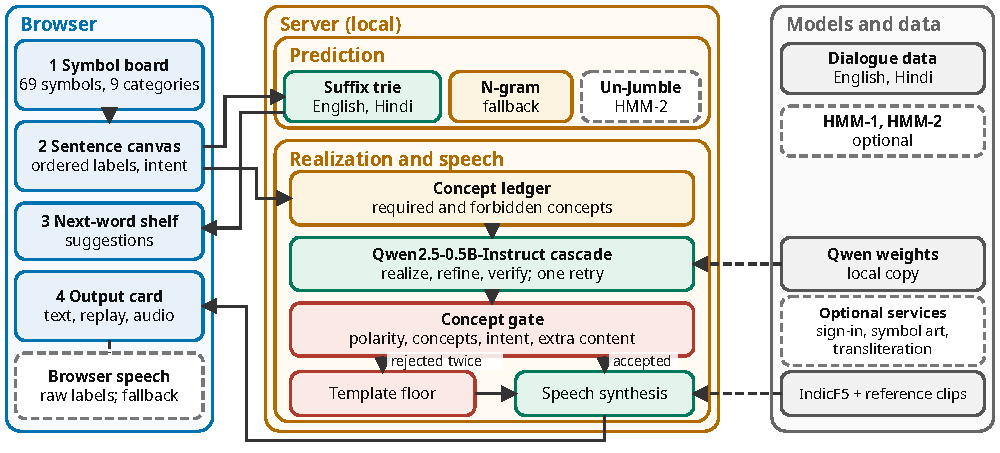
\includegraphics[width=0.92\textwidth]{figures/architecture.pdf}
\caption{Architecture of \sys{}. A selection in the browser goes to the server for next-word suggestions and for realization. The cascade output is spoken only if the gate accepts it; after two rejections a template built from the user's labels is spoken. Dashed boxes are optional components.}
\label{fig:arch}
\end{figure*}

\paragraph{Walkthrough.}
The user picks a language and taps symbols from a board of \NSymbols{} symbols in \NCategories{} categories, labeled in English, Hindi, Gujarati, and Marathi (Figure~\ref{fig:ui}, \cn{1}); free text, emoji search, and a personal ``My Words'' grid extend the vocabulary.
Selections accumulate on a sentence canvas (\cn{2}), and a shelf proposes next words with their probabilities (\cn{3}).
\emph{Speak} voices the literal labels with the browser's speech synthesis and needs no model round trip.
\emph{AI Polish \& Speak} (\cn{4}) sends the selection to the server, which returns a sentence that the output card shows while it is spoken (\cn{5}); the card offers Replay, Copy, and a bookmark for a one-tap Quick Picks shelf.
A Quick Express row speaks emergency phrases (Help, Water, Bathroom, Pain) in one tap, Un-Jumble reorders canvas words with a second HMM, and an accessibility dock adjusts card and text size, contrast, grayscale, and speech speed.

\begin{figure}[t]
\centering
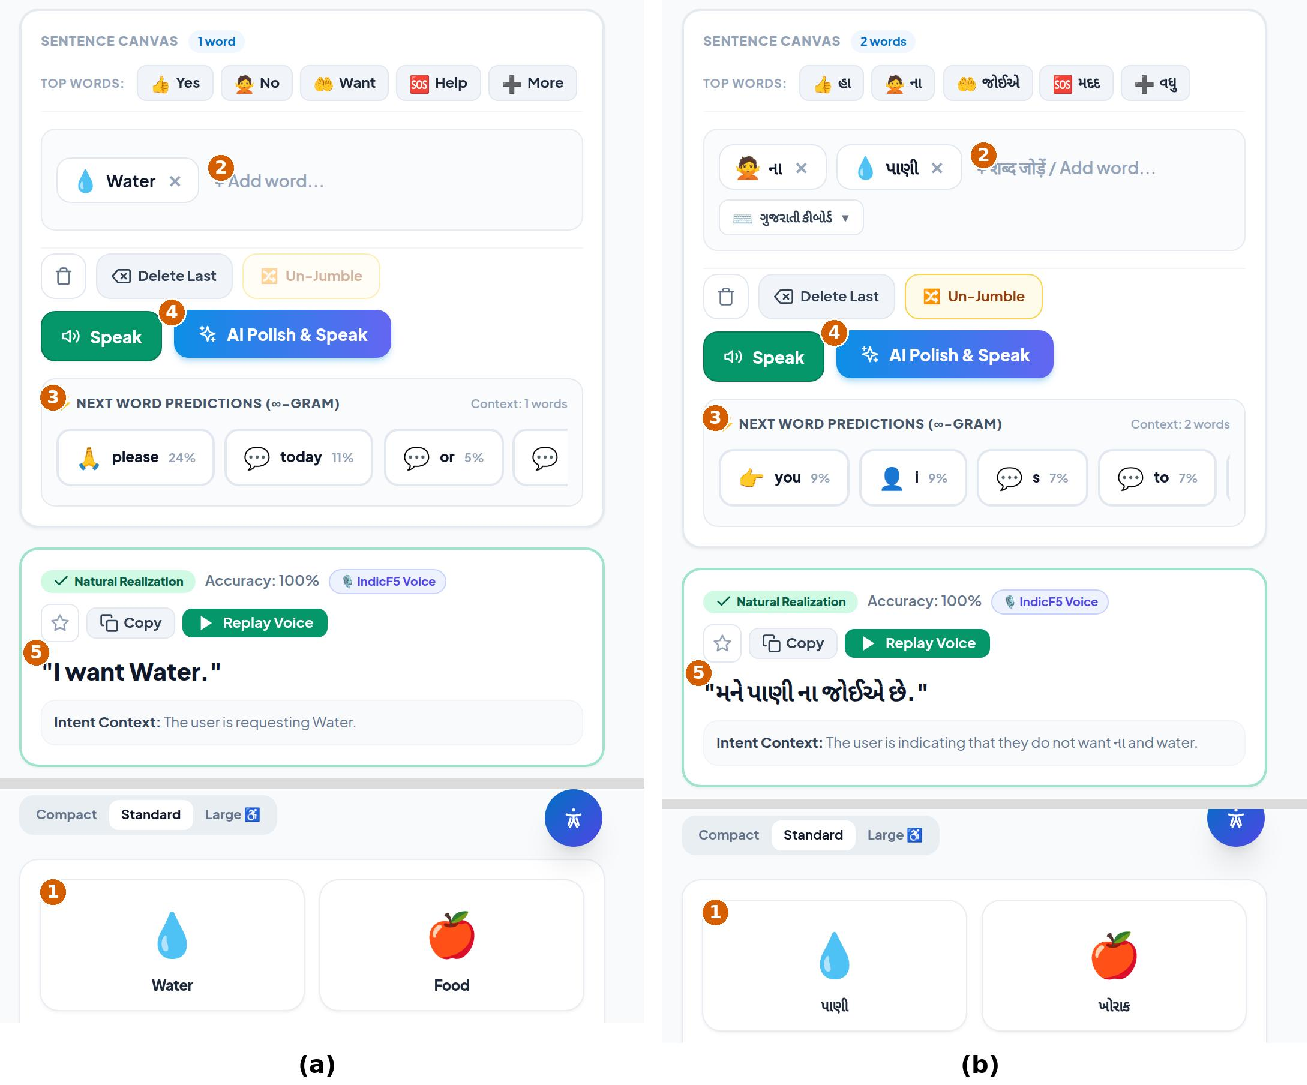
\includegraphics[width=\columnwidth]{figures/ui_panel.pdf}
\caption{The running build (Chrome, 520\,px viewport). (a)~English \emph{Water}: the cascade output was rejected and the template was spoken. (b)~Gujarati \gu{ના}\,+\,\gu{પાણી} (\emph{no}\,+\,\emph{water}): the cascade output was accepted. Callouts: \cn{1} symbol, \cn{2} canvas, \cn{3} next-word shelf, \cn{4} generate, \cn{5} output. The \emph{Accuracy} badge is the validator's heuristic score, not a gate threshold.}
\label{fig:ui}
\end{figure}

\paragraph{Request and concept ledger.}
The browser sends the ordered labels with the communicative intent (request, statement, question, or negation), a negation indicator, the language, and an optional code-mixing indicator.
The web client infers intent and negation from label substrings: negation if a label contains \emph{no}, \emph{not}, or a Hindi, Gujarati, or Marathi negator; question for question words; statement for a few feeling labels; request otherwise.
Any other client can supply both fields explicitly.
The server builds a \emph{ledger}: a required set (intent, speaker, each selected concept, negation) and a forbidden set of 21 default words for unrequested times, meals, and venues, minus any word the user selected.

\paragraph{Realization and gate.}
Three prompted stages share one frozen Qwen2.5-0.5B-Instruct \citep{qwen2025qwen25}.
The realizer writes a sentence from a few-shot prompt for Hindi, Gujarati, and Marathi (12, 9, and 9 examples; greedy decoding) and from a ledger prompt for English and code-mixed output (temperature 0.1); the refiner removes unsupported content and is skipped for Indic-script candidates; the verifier returns a verdict and a minimal rewrite.
The gate then decides.
With $\nu$ the negation indicator, $E$ the selected concepts, $F$ the forbidden set, and $y$ the candidate,
\begin{equation}
\begin{split}
\mathrm{acc}(y)={}&[\mathrm{neg}(y)=\nu]\wedge\mathrm{match}(E,y)\wedge\mathrm{intent}(y)\\
&\wedge\neg\mathrm{forbid}_F(y)\wedge\neg\mathrm{time}(y).
\end{split}
\label{eq:gate}
\end{equation}
Here \emph{neg} tests a list of English, Hindi, Gujarati, and Marathi negators; \emph{match} requires every selected concept to appear (a substring, plural, and Indic-stem test); \emph{intent} rejects ``I want'' for feeling intents and requires a question cue for questions; \emph{forbid} matches words of $F$; and \emph{time} flags time words when none was selected.
The verifier's verdict is advisory, and only the gate decides.
A rejection triggers one more cascade run, and after two rejections a language-specific template built from the selected labels (e.g., ``I want Water.'') is returned.
English and code-mixed retries resample, whereas greedy Indic retries repeat.

\paragraph{Prediction and speech.}
Next-word suggestions come from an unbounded-order suffix trie in the spirit of infini-gram \citep{liu2024infinigram}: contexts of any length are matched by suffix, and scores combine with backoff 0.4.
The trie is built in under a second at start-up from the English and Hindi AAC dialogues (\IGSent{} sentences, maximum depth \IGDepth{}); two HMMs trained on streamed text (HMM-1 for next words, HMM-2 for Un-Jumble) are optional components that the evaluated build ran without (Section~\ref{sec:limits}).
The returned sentence is synthesized by IndicF5 \citep{ai4bharat2025indicf5}, a flow-matching model of the F5-TTS family \citep{chen2025f5tts}, with a 24\,kHz Vocos vocoder \citep{siuzdak2023vocos}.
A reference clip and its exact transcript condition the voice zero-shot, so a caregiver can register a familiar voice.

\paragraph{What is trained.}
Qwen2.5-0.5B-Instruct is prompted, not fine-tuned, and IndicF5 is used as released.
We train the suffix trie and a Hindi HMM on the AAC dialogues, two HMMs on streamed English text, and an English Flan-T5 refiner (Appendix~\ref{app:models}).
